\chapter{Design}

\section{Hardware Design}
Proposed system will consist from the Raspberry Pi minicomputer(RPi), analogue inclinometer, gpio14 chip, a bunch of relays and the PTU.

\subsection{RPi}

 
As a main control unit by the client, where all the software will be running, was chosen the Raspberry Pi minicomputer. It will replace currently employed for this task Gumstix single board computer which provides limited control over the PTU. 

RPi is a credit-card-sized single-board computer with a 512 MiB of RAM and 700 MHz ARM based CPU. It is powerful enough for the proposed tasks and have all the required interface to be connect to the other peripheral. In particular it has GPIO pins including, SPI and I$^2$C interfaces, UART serial console, 5v and GND supply pins. Such powerful devices for this task may be an overkill, but decision was made by the client and I work with what I have.

\subsection{Inclinometer}
Inclinometer will be used to get data about the current chassis position in the space. Client suggested usage of the SCA121T dual axis inclinometer (figure~\ref{fig:SCA121T-D05_inclinometer}) bolted to the chassis of the rover. It will provide information about the inclination angles during calibration. Since it is a analogue device we will need a A/D converter. 

\begin{figure}[H]
\centering
\centerline{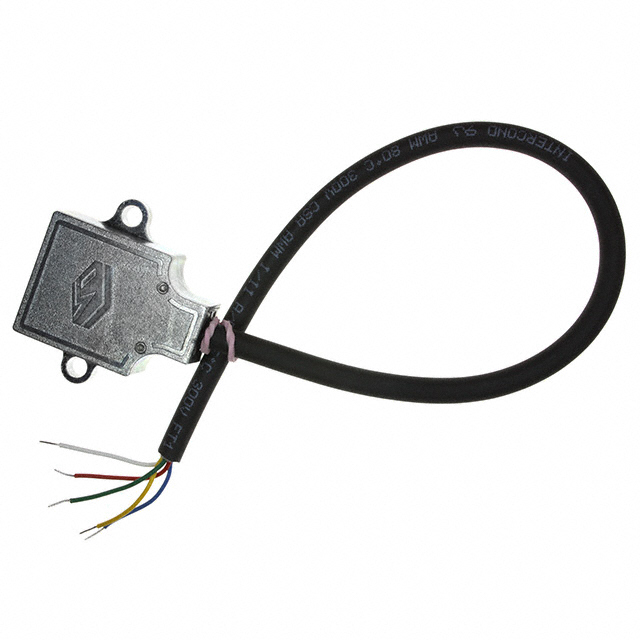
\includegraphics[scale=0.20]{./images/SCA121T}}
\caption{SCA121T-D05 Inclinometer}
\label{fig:SCA121T-D05_inclinometer}
\end{figure}

\subsection{GPIO14 chip}
The GPIO14 chip is a pre-programmed PIC16F818 micro controller. It is intended to provide general purpose I/O expansion on the $I^2$C bus. It has 14 general purpose I/O lines and 5 analogues input channels with 10-bit A/D conversion \cite{GPIO14}. GPIO14 chip will be used to convert inclinometer signal from the analogue format to digital and switch on/off relays. This chip will be connected over the I$^2$C bus to the RPi.

\subsection{PTU}
Pan-and-Tilt Unit is a high-precision integrated motion control systems produced by the Sagebrush Technology (now part of the RIEtech Global, LLC \cite{RIEtech_Global}). It is designed for the <10Kg payloads and typically is used to hold cameras, antennas or instrument positioning. In this projects it is used to hold a panoramic camera. 

\section{Software Design}
My work will be based on the code that is already used on the Gumstix. Currently it is used to send control commands to the PTU, get readings from the inclinometer and switch on/off relays. The code base have three main parts in it. The client side software, server side software (running on the Gumstix and responding to client calls) and the library that implements TASS protocol. 

\subsection{TASS library}
TASS library implements the protocol to communicate with the PTU. All communication is done over the RS-232 interface. To connect it to the RPi (which has TTL interface) was used RS-232-TTL converter. Currently this library has support for the basic commands like pan left/right, tilt up/down, get/set position, get/set rotation limits.

My task is to add implementation for the stabilize and drift rate commands as well as logic for the drift rate calculation.

\subsection{Server Side}
The server side software is responsible for the overall control of the PTU and inclinometer, it will be running on Raspberry Pi minicomputer and will respond to the client commands. On of the main challenges is to port current system from the Gumstix to the RPi platform and make it to work.

\subsection{Clint Side}
The client side software provides an API to interact with the server Side. Connection is done over the TCP/IP protocol. The plan is extend API upon the creation of the new stabilization functionality. 

\subsection{Operating System}
Raspbian is a free operating system that will be running on the RPi. It requires some initial configuration before the main software can be successfully run. In particular it requires some configuration to prevent Linux from using the serial port and it also needs WiringPi library \cite{WiringPi} to be installed to successfully communicate over the I$^2$C bus with the GPIO14 chip. All necessary configuration is covered in Appendix A.  

\section{Overall Architecture}


\section{Some detailed design}

\subsection{Even more detail}

\section{User Interface}

\section{Other relevant sections}